\chapter{Simulations with the \pkg{specsim} package}

Introduction: used to generate simulations for eBOSS Lyman-alpha and to verify DESI sky model. 

\section{Spectroscopic simulations with \pkg{specsim}}

\pkg{specsim} \cite{Kirkby_21} is a software package developed by Dr. David Kirkby to simulate the response of a multi-fiber spectrograph. Although it was originally created to generate realistic synthetic spectra for the DESI instrument, it can be reconfigured to simulate any fiber-fed spectrograph, provided that the accompanying instrument parameter specifications and data are provided.

A single simulation consists of three components: a source spectrum, a model of the sky and atmosphere, and a model of the instrument. A schema of where each component comes into play is shown in Fig. \ref{fig:schema}, which shows the journey of photons as they are emitted from a galaxy to the moment they are read out by the detector.

\begin{figure}[h]
\centering
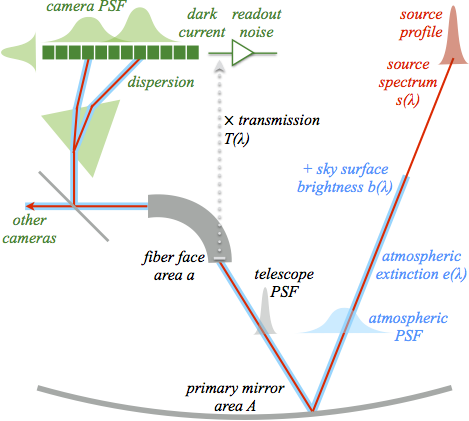
\includegraphics[width=11cm]{images/specsim/overview.png}
\caption{Specsim schema.}
\label{fig:schema}
\end{figure}

\subsection{Astrophysical source}
% Needs work/editing
Spectra of astrophysical sources are simulated individually, beginning with a spectral energy distribution (SED) in its rest frame, $s(\lambda)$, and its morphological profile. Configuration parameters for a source profile include the bulge/disk fraction and shape parameters such as the half-light radius, position angle, and the ratio of the semi-minor to semi-major axis. The source profile is assumed to be independent of its SED, and will come into play later on when accounting for fiberloss when modeling the effects of the instrument.

\begin{table}[h]
\caption{Specsim simulation parameters.}
\label{tab:specsim_vars}
\centering
\begin{tabular}{|c|c|c|}
  \hline
  Parameter & Component & Description \\
  \hline \hline
  $\Delta t$ & Instrument & Exposure time \\
  \hline
  $X$ & Atmosphere & Observing airmass \\
  \hline
  $\lambda_{i}$ & Configuration & Fine wavelength grid \\
  \hline
  $s(\lambda)$ & Source & Source SED \\
  \hline
  $b(\lambda)$ & Atmosphere & Sky surface brightness \\
  \hline
  $e(\lambda)$ & Atmosphere & Atmospheric extinction \\
  \hline
  $A$ & Instrument & Primary unobscured area \\
  \hline
  $a$ & Instrument & Fiber entrance area \\
  \hline
  $f_{S}(\lambda)$ & Source \& Instrument & Fiberloss fraction \\
  \hline 
  $T_{i}(\lambda)$ & Camera & Transmission throughput \\
  \hline
  $d_{i}(\lambda)$ & Camera & CCD row width \\
  \hline
  \sigma_{i}(\lambda) & Camera & CCD resolution \\
  \hline
  $n_{ip}$ & Camera & CCD trace width \\
  \hline
  $I_{dk,i}$ & Camera & Sensor dark current \\
  \hline
  $G_{i}$ & Camera & CCD gain \\
  \hline
  $\sigma_{ro,i}$ & Camera & Readout noise \\
  \hline
\end{tabular}
\end{table}

\subsection{Sky model}
Given a source, the next component of the \pkg{specsim} pipeline is the sky model, which incorporates the effects of the atmosphere. The three elements that make up the sky model are a sky emission spectrum, the atmospheric point spread function, or PSF, and atmospheric extinction.

% Include side-by-side plots of DESI vs eBOSS dark sky here
% Talk about downsampling?

% Sky emission
The sky model used for both DESI and eBOSS configurations is virtually identical. The sky emission surface brightness $b(\lambda)$ for the DESI configuration contains data for three different types of sky spectra corresponding to dark, bright and grey conditions, whereas the eBOSS sky emmission spectrum is just the DESI dark sky extrapolated to cover the wider wavelength range of the eBOSS spectrograph.

% Seeing
Atmospheric PSF results in the blurring of an image of a source as its photons encounter varying indices of refraction when traveling through different layers of the Earth's atmosphere. Differences in temperature, pressure, density and molecular composition in each layer, as well as turbulence in the air, cause photons to slightly deflect from their original paths, resulting in a ``smeared" image. Seeing is defined as the full width at half maximum (FWHM) of a radial profile of a point source, typically a star, from its peak value.

The effects of atmospheric seeing in \pkg{specsim} can be applied in one of three ways. The fastest mode assumes a fixed 1.1" seeing for each source type (LRG, ELG, QSO, etc.), and doesn't account for any additional information about surface brightness profiles. A slower, but more flexible mode uses \pkg{GalSim}, a package that simulates images of astrophysical sources (cite), to convolve the source profile with the atmospheric PSF. \pkg{GalSim} requires additional information in the configuration file such as FWHM$_{ref}$ and $\lambda_{ref}$, which are used to estimate the PSF as a function of wavelength in the following way:

\begin{equation}
    \mbox{FWHM}(\lambda) = \mbox{FWHM}_{ref} \Big(\frac{\lambda}{\lambda_{ref}}\Big)^{-0.2}.
\end{equation}

Since \pkg{GalSim} uses a Moffat profile to model the PSF, a fixed value for the $\beta$ parameter, which determines the shape of the PSF, must also be specified. The Moffat distribution is predominantly used for modeling PSFs as it is more successful at capturing tails compared to a Gaussian or Lorentzian distribution.

The final component in the sky model is atmospheric extinction, which could be caused by Rayleigh scattering of air molecules or particulate matter such as aerosols, or by telluric absorption due to the Earth's atmosphere. This is provided in the configuration file as a list of tabulated values for the extinction coefficient $e(\lambda)$ at zenith as a function of wavelength. The amount of extinction at other airmasses is determined by multiplying the the extinction coefficient by the airmass at that particular pointing.

Together, the three components of the sky model can be combined to model the attenuation of the source and emission spectra in terms of the extinction factor $-e(\lambda)$ and the airmass $X$ due to the effects of the atmosphere: 

\begin{equation}
    10^{-e(\lambda)X/2.5}.
\end{equation}

\pkg{specsim} allows the option to include a scattered moonlight component as part of the sky brightness spectrum, which is determined for each observation by a solar SED (given by http://rredc.nrel.gov/solar/spectra/am0/), the moon phase, the moon zenith and the separation angle between the telescope pointing and the moon.

\subsection{Telescope and instrument}

\subsubsection{Telescope}
Once the light from a source has completed its passage through the atmosphere, it finally begins the final leg of its journey when it enters the telescope and is registered by the detector.

Photons that are incident on the telescope are impacted by the total collecting area of the primary mirror, $A$, used to normalize both the source flux and the sky brightness. Unlike the source spectrum, the sky level is proportional to the size of the fiber, and therefore must also be normalized by the fiber face area $a$. The telescope has an optical PSF which is due to the diffraction of light by the telescope aperture and potential aberrations in the lens or mirror. In a diffraction-limited system, the telescope will have reached its theoretical limit and the only contribution to the optical PSF will be due to the finite size of the aperture. This PSF is convolved with the atmospheric PSF and the source profile to determine the fiberloss $f_{S}(\lambda)$, or the fraction of photons incident on the fiber face that make it through the fiber (see Section \ref{sec:instrument}). The flux density of the source is transformed to give the flux in units of $erg / \AA$ up to the point just before the photons enter the camera: 

\begin{equation}
    F(\lambda) = 10^{-e(\lambda)X/2.5}\Big[s(\lambda) + ab(\lambda)\Big]f_{S}(\lambda)A\Delta t,
\label{eq:flux}
\end{equation}

where $\Delta t$ is the length of a single exposure. The last step after combining the impacts of the atmosphere and telescope is to simulate the effects of the camera.

\subsubsection{Instrument}
\label{sec:instrument}
\pkg{specsim} is able to simulate the response of a spectrograph and one or more cameras. This involves characterizing the effects of the instrument once photons have exited the fiber, as shown in the green portion of Fig. \ref{fig:schema}, beginning with the dispersion $d_{i}(\lambda)$, indexed by camera $i$, as incoming light is separated into its constituent wavelengths by the spectrograph. This is also referred to as the row width, and gives the conversion from wavelength in Angstroms to size in pixels.

Once the light has been converted into a spectrum, it reaches one or more detectors, or charge-coupled devices (CCDs) (see Chapter 2), where it is registered as a function of fiber number along the vertical direction, and wavelength or pixel number along the horizontal axis. If one were to plot a distribution of where photons from a single source landed on the detector, as a function of wavelength, the CCD resolution $\sigma_{i}(\lambda)$ would correspond to the Gaussian sigma of the best-fit Gaussian to that distribution. Values for the trace width, which gives the thickness of the spectrum on the fiber axis, corresponding to the read noise in the spatial direction, must also be provided in the configuration file. Additional values for the amount of dark current, read noise, gain and throughput for each camera must also be specified. Further details regarding each of these parameters will be given in the following section.

The calculations used to determine the camera response are performed on a simulation grid $\lambda_{j}$ (indexed by bin $j$) whose resolution is greater than the wavelength extent of a single camera pixel by at least a factor of five. If a photon with wavelength $\lambda_{j} < \lambda < \lambda_{j+1}$ enters a fiber and lands in a bin of width $\Delta \lambda_{j}$, where

\begin{equation}
    \Delta \lambda_{j} \equiv \lambda_{j+1} - \lamda{j}\,,
\end{equation}

then the energy $E_{j}$ associated with this photon in ergs can be derived from the Planck equation:

\begin{equation}
    E_{j} = \frac{hc}{\Delta \lambda{j}}\,,
\end{equation}

where $h$ is Planck's constant and $c$ is the speed of light. This can be used to convert from the flux density in Eq. \ref{eq:flux} at the center of each bin to the number of photons entering the fiber $N_{j}^{\gamma}$:

\begin{equation}
    N_{j}^{\gamma} = \frac{\Delta \lambda_{j}}{hc\bar{\lambda}_{j}}F(\bar{\lambda}_{j}).
\end{equation} 

The bin centers are given by:

\begin{equation}
    \bar{\lambda}_{j} \equiv \frac{\lambda_{j+1} - \lambda_{j}}{2}\,.\\
\end{equation}

Each camera's throughput $T_{i}(\lambda)$ is defined as the probability that a photon incident on a fiber is converted into a photo-electron and registered by the CCD. The resolution effects in the wavelength direction $\sigma_{i}$ is given by a convolution matrix $R_{jk}$, taking us from the simulation grid indexed by $j$ to a detection grid indexed by $k$. Adding the effects of camera throughput and summing over the simulation pixels gives the number of detected electrons for camera $i$ as a function of pixels in the detection grid:

\begin{equation}
    N_{ik}^{e} = \sum_{j}R_{jk}N_{j}^{\gamma}T_{i}(\lambda_{j})\,.
\end{equation}

%what is N^{eh} in specsim docs?

Next, the dispersion function $d_i(\bar{\lambda}_{k})$ is determined as a function of Angstroms in the detection grid in order to re-bin the number of detected counts from the detection wavelength grid to continuous pixel coordinates $N_{ip}^{e}$.

Folding in sensor effects such as the camera gain $G_{i}$ and dark current $I_{dk,i}$ gives the signal in terms of the number of detected electrons:

\begin{equation}
    N_{ip}^{det} = G_{i}N_{ip}^{e} + I_{dk,i}n_{ip}\Delta t\,,
\end{equation}

where $n_{ip}$ is the trace width in pixels for wavelength pixel $p$. The variance of the resulting signal is given by:

\begin{equation}
    V_{ip}^{det} = N_{ip}^{det} + \sigma_{ro,i}^{2}n_{ip}\,,
\end{equation}

where $\sigma_{ro,i}$ is the readout noise in pixels. The read noise is assumed to be uncorrelated between pixels.

%"The source flux is integrated over the fiber, but the sky spectrum is a "surface brightness" so has an extra "/sq.arcsec." in its units, so needs to be multiplied by the fiber area. Think of a really big fiber: the rate of source photons would be independent of the fiber size, since they are 100% collected (FFRAC=1), but the rate of sky photons scales with the fiber area."

\section{Simulating the eBOSS instrument response}

% synthetic, mocks, simulations

% Intro
The \pkg{specsim} package was developed with the flexibility to simulate the response of any multi-fiber spectrograph, given that the accompanying configuration data is provided. There were several motivations for reconfiguring \pkg{specsim} to simulate the eBOSS instrument and cameras. Firstly, an eBOSS configuration would serve a critical purpose by allowing for the validation of \pkg{specsim} itself, since eBOSS data already exists. From a software engineering perspective, it would confirm the extent to which the package is in fact generalizeable. Although the package should in theory be able to extend to other instruments, this had never actually been done before -- \pkg{specsim} had only been set up to produce synthetic DESI spectra, and it was unclear how difficult it would be to accommodate two spectrographic arms for eBOSS instead of three for DESI, or to use different wavelength binnings, among other things. Another useful application, and the primary motivation for this undertaking, was to generate realistic simulations of eBOSS spectra for the eBOSS Lyman-$\alpha$ working group.

\subsection{Generation of mocks for Lyman-alpha studies}

% Brief background on Lyman-alpha working group studies

Baryon acoustic oscillations (BAO, see Intro section xx) originating from the pre-recombination universe are a cosmological ``standard ruler" whose imprints are seen as peaks in the matter correlation function at the sound horizon. Measurements of the BAO scale can be measured from the clustering of galaxies for redshifts below $z<2$, but there are simply not enough tracers at redshifts above this limit for high-precision clustering measurements. The alternative is to use opacity fluctuations due to the absorption of neutral hydrogen in the Lyman-$\alpha$ forest of background quasars. The final eBOSS data release, Data Release 16, includes all quasars observed by both BOSS and eBOSS, including 210,005 quasars above $z>1.10$ \cite{du_Mas_des_Bourboux_2020}.

The eBOSS Lyman-$\alpha$ working group rely on faithful representations of quasar spectra to validate analysis pipelines and study potential sources of systematic effects \cite{Farr_2020}. Mock quasar spectra specifically generated with the eBOSS configuration of \pkg{specsim} were used to estimate the detection efficiency of Damped Lyman-$\alpha$ systems using a convolutional neural network, ultimately revealing the purity of the quasar sample used for BAO studies \cite{Chabanier_21}. 

The production of mocks begins with the generation of a Gaussian random field on a box of length 10 $h^{-1}$ Gpc. The peaks of this physical density field are then populated with tracer quasars via Poisson sampling, based on an input bias and number density. Next, skewers for each quasar are generated by interpolating the density field along the line-of-sight, and then processed to convert from fluctuations in the density field to a transmitted flux fraction for each Lyman-$\alpha$ spectrum \cite{du_Mas_des_Bourboux_2020}. These processed skewers are the source inputs to \pkg{specsim}, as shown in the red portion of Fig. \ref{fig:schema}.

% We present the characteristics of the Damped Lyman-α (DLA) systems found in the data release DR16 of the extended Baryon Oscillation Spectroscopic Survey (eBOSS) of the Sloan Digital Sky Sur- vey (SDSS). DLAs were identified using the convolutional neural network (CNN) of Parks et al. (2018). A total of 117,458 absorbers candidates were found with 2 ≤ zDLA ≤ 5.5 and 19.7 ≤ log N (HI ) ≤ 22, including 57,136 DLA candidates with log N (HI ) ≥ 20.3. Mock quasar spectra were used to estimate DLA detection efficiency and the purity of the resulting catalog. Restricting the quasar sample to bright forests, i.e. those with mean forest fluxes fλ > 2 × 10−19 W m−2 nm−1, the completeness and purity are greater than 90% for DLAs with column densities in the range 20.1 ≤ log N (HI ) ≤ 22.

% Helion: Apart from the statistical gain from new quasars and deeper observations, the main improvements over previous work come from more accurate modeling of physical and instrumental correlations and the use of new sets of mock data.Two new sets of three-dimensional (3D) Gaussian random field simulations have been developed to char- acterize our combined measurement of the auto- and cross-correlation (see Section 5). These mocks allow us to test the steps of the data analysis, thus study potential sources of systematic errors and test the estimation of statistical errors. Unlike our previous mock spectra, the Lyβ spectral region is also simulated and studied.

% Farr (https://arxiv.org/pdf/1912.02763.pdf): Generating mock datasets for such measurements will be important for validating analy- sis pipelines and evaluating the effects of systematics. With such studies in mind, we present LyaCoLoRe: a package for producing synthetic Lyman-α forest survey datasets for BAO anal- yses. LyaCoLoRe transforms initial Gaussian random field skewers into skewers of transmitted flux fraction via a number of fast approximations. 
% The upcoming Dark Energy Spectroscopic Instrument (DESI) [27] will be able to ad- vance these measurements greatly. Over the 5 years of its operation, it will measure approx- imately 800,000 QSO spectra with z > 2.0, 3 times as many as in the final eBOSS dataset (approximately 270,000). Ahead of such an increase in statistical power, it is vital to be able to sufficiently test analysis pipelines to ensure that they do not introduce any biases. Equally, it is important to be able to quantify exactly how secondary astrophysical effects will impact upon BAO measurements. The best way to carry out both of these tests is through the development of mock datasets [e.g. 28–30] — synthetic realisations of a survey for which cosmological and astrophysical parameters can be easily controlled. 
% Having generated a physical density field, tracers such as QSOs can be placed at its peaks via Poisson sampling according to an input bias and number density, and line-of-sight skewers can be drawn by interpolating within the box. Converting density skewers to mimic the transmitted flux fraction of the Lyα forest then requires a significant degree of post-processing.
% In this work, we use CoLoRe [37] to generate our initial Gaussian skewers, as described in § 2.1. We then present the package LyaCoLoRe, which is able to convert CoLoRe’s output into realistic skewers of transmitted flux fraction. The output skewers from LyaCoLoRe then require the addition of instrumental noise and combination with a QSO continuum before they can be considered realistic spectra. This can be carried out in the context of DESI by a package called desisim1, which is not discussed in this work.
% The primary motivation for creating the LyaCoLoRe mocks is to provide realistic sets of test skewers for BAO analyses from Lyα forest surveys. Evidently then, it is important to verify that the fundamental physical quantities studied by such analyses are correctly reproduced in the mock datasets. We thus seek to test that the BAO signal is present and unbiased in our mock datasets. 
% Talk about eBOSS data
% See Smee paper for details?
% Mention downsampling in eBOSS and making output eBOSS wlen grid linear in log-lambda to match eBOSS format

\subsection{Instrument parameters}

A new configuration file was produced for the eBOSS instrument and named \pkg{sdss.config}. Values for the fixed telescope parameters were added, which included the size of the primary mirror, the obscuration diameter (the size of the gap in the primary mirror where light reflected off of the secondary mirror passes through), the size of the fibers, and the field radius (the radius of the plate). The read noise, dark current and gain for each camera, which contribute to added noise in the camera, were also specified. Values for both the DESI and eBOSS telescope and camera parameters as they appear in their respective configuration files are shown in Tables \ref{tab:comparison}-\ref{tab:ebosscam}.\\

\begin{table}[h]
\caption{Telescope parameters: DESI vs eBOSS.}
\label{tab:comparison}
\centering
\begin{tabular}{|c|c|c|}
  \hline
  Telescope Parameters & DESI & eBOSS\\
  \hline \hline
  Primary mirror diameter (m) & 3.797 & 2.5 \\
  \hline
  Obscuration diameter (m) & 1.8 & 0.625 \\
  \hline
  Fiber diameter ($\mu m$) & 107.0 & 120.0 \\
  \hline
  Field radius (mm) & 414.0 & 325.0 \\
  \hline
\end{tabular}
\end{table}

\begin{table}[h]
\caption{DESI camera parameters.}
\label{tab:desicam}
\centering
\begin{tabular}{|c|c|c|c|}
  \hline
  Camera parameters & b & r & z\\
  \hline \hline
  Read noise (e$^{-}$/pixel$^{2}$) & 3.0 & 2.9 & 2.9 \\
  \hline
  Dark current (e$^{-}$/hour/pixel$^{2}$) & 3.0 & 2.0 & 2.0 \\
  \hline
  Gain (e$^{-}$/ADU) & 1.0 & 1.0 & 1.0\\
  \hline
\end{tabular}
\end{table}

\begin{table}[h]
\caption{eBOSS camera parameters.}
\label{tab:ebosscam}
\centering
\begin{tabular}{|c|c|c|}
  \hline
  Camera parameters & b & r\\
  \hline \hline
  Read noise (e$^{-}$/pixel$^{2}$) & 2.0 & 2.75 \\
  \hline
  Dark current (e$^{-}$/hour/pixel$^{2}$) & 2.1 & 4.25 \\
  \hline
  Gain (e$^{-}$/ADU) & 1.02 & 1.66\\
  \hline
\end{tabular}
\end{table}

\subsection{Camera}

Camera data was derived separately for the red and blue cameras using data from real eBOSS spectra. The \pkg{bossdata} software package \cite{xx} was used to download data from the Sloan Digital Sky Survey (SDSS) Sky Server, and was part of version \pkg{v5$_$9$_$0} of Data Release 13, the first data release of the fourth phase of SDSS (SDSS-IV). Data was pulled from 20 random plates, each observed on a different day, for all four cameras (two blue cameras, b1 and b2, and two red cameras, r1 and r2). 

% make this horizontal?
\begin{table}[h]
\caption{eBOSS plate, mjd data.}
\label{tab:eboss_plates}
\centering
\begin{tabular}{|c|c|}
\hline
  Plate & MJD \\
  \hline \hline
  7027 & 56448 \\
  \hline
  6963 & 56724 \\
  \hline
  7301 & 56746 \\
  \hline
  6759 & 56416 \\
  \hline
  6002 & 56104 \\
  \hline
  6178 & 56213 \\
  \hline
  6626 & 56330 \\
  \hline
  6882 & 56541 \\
  \hline
  7389 & 56769 \\
  \hline
  7453 & 56749 \\
  \hline
  7517 & 56772 \\
  \hline
  6472 & 56362 \\
  \hline
  6660 & 56370 \\
  \hline
  6877 & 56544 \\
  \hline
  6970 & 56444 \\
  \hline
  6122 & 56246 \\
  \hline
  7456 & 56727 \\
  \hline
  7377 & 56741 \\
  \hline
  7454 & 56751 \\
  \hline
  7564 & 56804 \\
  \hline
\end{tabular}
\end{table}

% Maybe make a note of how all data was produced in the same way, using all fibers on 20 different plates, interpolating data for each fiber over the canonical grid, and then taking the median of all 20 x 1000 fibers

\subsubsection{Wavelength binning}

The first task was to generate a canonical wavelength grid for each camera. Unlike the two other wavelength grids used in \pkg{specsim} (the wavelength solution for the source spectrum, controlled by the user, and a finely binned simulation grid with a resolution of 0.1$\mbox{\AA}$ is used to perform calculations for the instrument response), this canonical grid is the final wavelength binning of the simulated output. It is also the common grid over which the rest of the camera data in this section was interpolated over to be used in the configuration file. This canonical grid was derived by combining the wavelength data for the two cameras in each channel separately (b1 with b2, and r1 with r2), and generating a linear grid with equal 1$\mbox{\AA}$ binning with endpoints determined by the minimum and maximum wavelength values of all combined fibers on all plates. The wavelength solutions for all fibers on each camera are shown in Fig. \ref{fig:wavelength_solutions}, and the final result, shown in Fig. \ref{fig:canonical}, displays the output grids for each camera for both eBOSS and DESI configurations. Since the eBOSS pipeline stores spectra in units of log10($\mbox{\AA}}$), the final output employed a similar logarithmic wavelength sampling. This is discussed further in Section xx.\\

\begin{figure}[h]
\centering
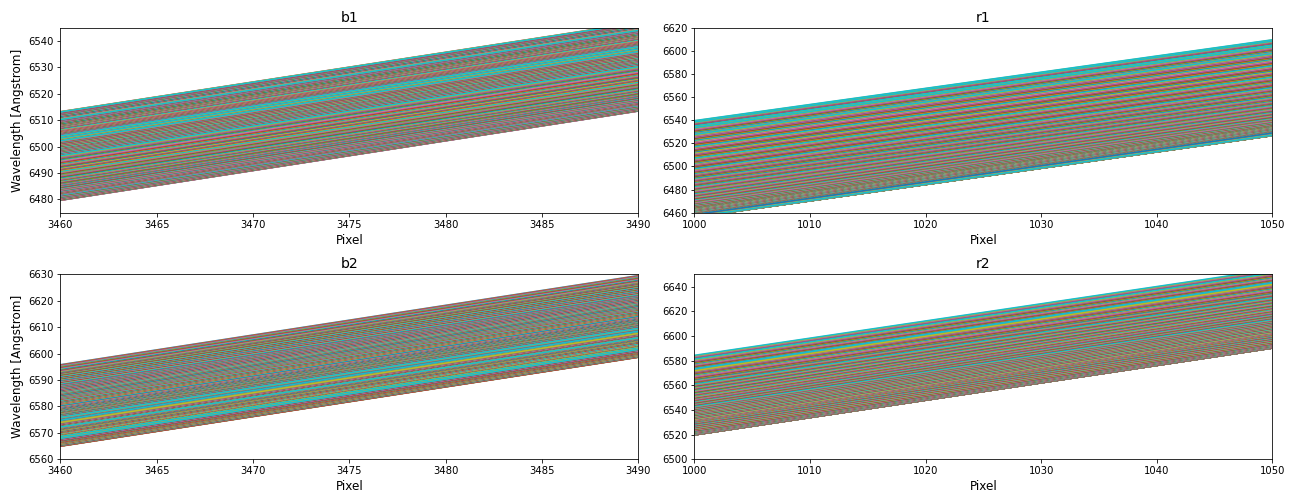
\includegraphics[width=16cm]{images/specsim/wlen_soln.png}
\caption{Wavelength solutions for all 500 fibers on each camera over 20 plates.}
\label{fig:wavelength_solutions}
\end{figure}


\begin{figure}[h]
\centering
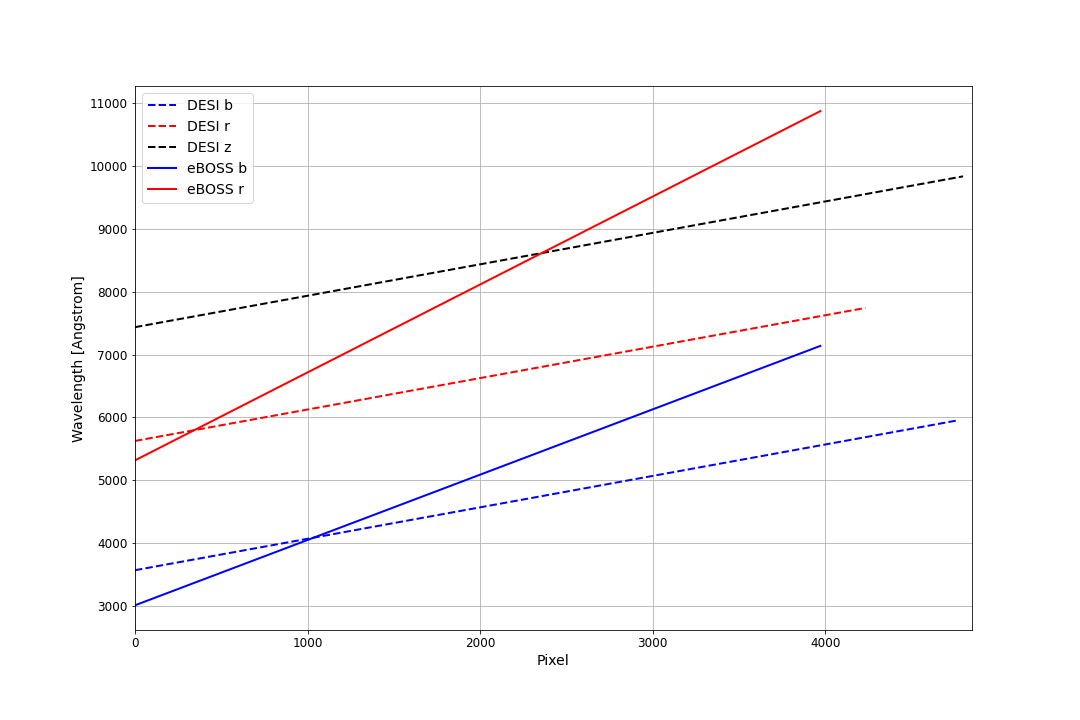
\includegraphics[width=14cm]{images/specsim/canonical_grid.png}
\caption{Canonical wavelength grids.}
\label{fig:canonical}
\end{figure}

\begin{figure}[h]
\centering
\begin{subfigure}[b]{0.55\textwidth}
   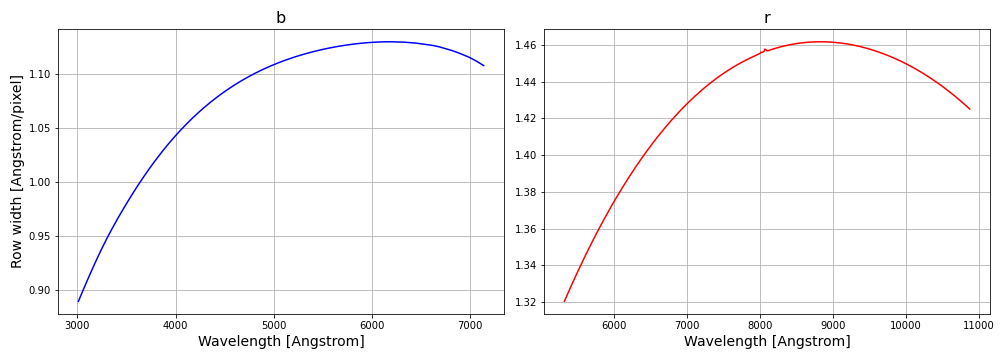
\includegraphics[width=14cm]{images/specsim/eboss_row_width.png}
   \caption{eBOSS dispersion.}
   \label{fig:eboss_disp} 
\end{subfigure}

\begin{subfigure}[b]{0.55\textwidth}
   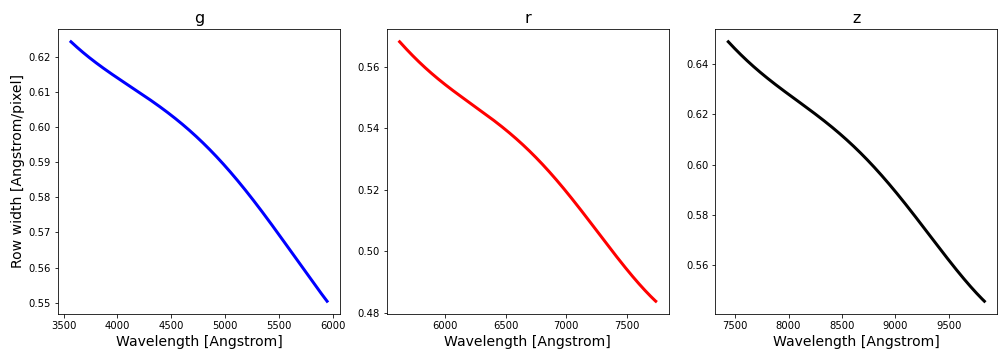
\includegraphics[width=14cm]{images/specsim/desi_row_width.png}
   \caption{DESI dispersion.}
   \label{fig:desi_disp}
\end{subfigure}
\caption[Two numerical solutions]{(a) Describe top figure. (b) Describe bottom figure.}
\label{fig:disp}
\end{figure}

\subsubsection{Spectral resolution}

The wavelength solution, dispersion and FWHM resolution for each fiber were accessed from \pkg{spCFrame} files. These files contain flux-calibrated spectra for a single camera of a single exposure. The dispersion was determined by taking the gradient of the wavelength solution with respect to wavelength. The FWHM resolution, was provided in the files and converted from units of 10$^{-4}$ log10($\mbox{\AA}$) and to Angstroms.

Spatial resolution data was obtained from \pkg{spFlat} files as the first-order corrected profile width for each fiber bundle. The Gaussian sigma for this profile, given in units of pixels, came in the form of a trace, or table of coefficients as a function of $x-$position on the CCD, that were then fed to a fitting function. This gave the spatial width as a function of wavelength.

Data for the dispersion, FWHM resolution, and spatial resolution were combined in the same fashion. After combining the data for each blue or red camera, these quantities were interpolated separately for all fibers over the canonical grid, and the median over all fibers and all plates was taken. The final results, along with DESI values for comparison, are shown in Figs. \ref{fig:disp}-\ref{fig:neff}.

% Need picture showing pixel vs fiber direction

\begin{figure}[h]
\centering
\begin{subfigure}[b]{0.55\textwidth}
   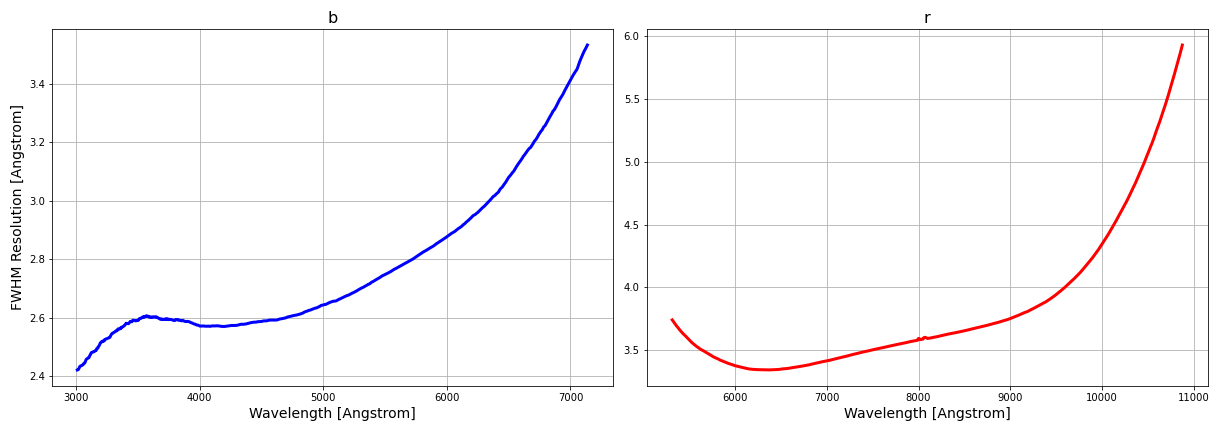
\includegraphics[width=14cm]{images/specsim/eboss_resolution.png}
   \caption{eBOSS FWHM resolution.}
   \label{fig:eboss_fwhm} 
\label{fig:fwhm}
\end{subfigure}

\begin{subfigure}[b]{0.55\textwidth}
   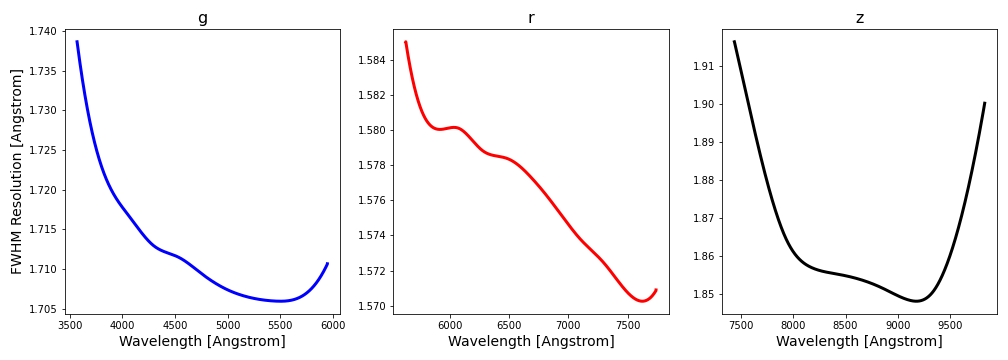
\includegraphics[width=14cm]{images/specsim/desi_resolution.png}
   \caption{DESI FWHM resolution.}
   \label{fig:desi_fwhm}
\end{subfigure}
\caption[Two numerical solutions]{(a) Describe top figure. (b) Describe bottom figure.}
\end{figure}

\begin{figure}[h]
\centering
\begin{subfigure}[b]{0.55\textwidth}
   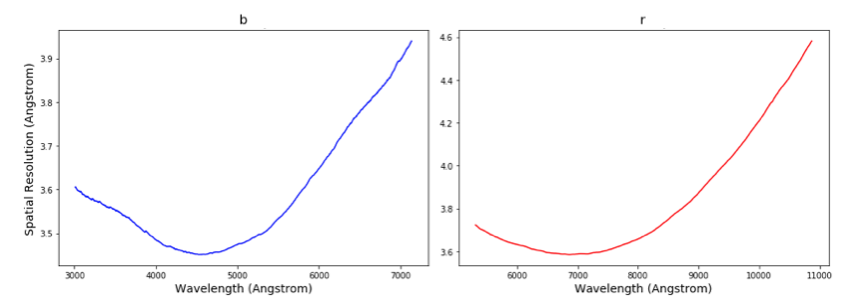
\includegraphics[width=14cm]{images/specsim/eboss_neff.png}
   \caption{eBOSS spatial resolution.}
   \label{fig:eboss_neff} 
\end{subfigure}

\begin{subfigure}[b]{0.55\textwidth}
   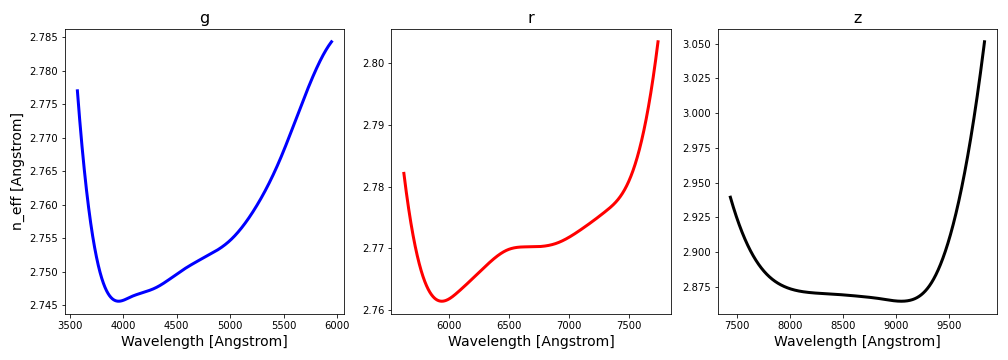
\includegraphics[width=14cm]{images/specsim/desi_neff.png}
   \caption{DESI spatial resolution.}
   \label{fig:desi_neff}
\end{subfigure}
\caption[Two numerical solutions]{(a) Describe top figure. (b) Describe bottom figure.}
\label{fig:neff}
\end{figure}


\subsubsection{Throughput}

Throughput data was initially generated for eBOSS quasars by working backwards from flux-calibrated SEDs to detected electrons. The SEDs were derived from all standard stars on the plates in Table \ref{tab:eboss_plates}. Standard stars were used because, like quasars, their profiles are PSF-like. Since they are brighter, they also have a higher signal-to-noise ratio. 

Fig. \ref{fig:fiberloss_chart} shows the process of going from the final, calibrated flux, to the product of fiberloss and throughput for a single standard star. This product is the ratio of detected electrons on the CCD to photons entering the telescope. The top four panels trace the process of obtaining the number of photons using data from \pkg{spFrame} files, which contain non-calibrated spectra for a single exposure of an individual camera. The bottom four chart show the number of incoming photons is derived using data from \pkg{spCFrame} files.

We begin with a flux density in the upper left panel, which has been interpolated over the nominal wavelength grid. We then convert from a density to the number photons above the atmosphere by multiplying by the area of the primary mirror, the exposure time, and dividing by the energy of each photon at the midpoints of the canonical wavelength bins. Next we must remove the extinction correction, shown in the third panel, interpolated over the nominal grid. This is done by multiplying the photons entering the atmosphere by the extinction to give the number of photons entering the telescope. 

To derive the number of electrons detected by the camera, we start with the flux in flat-fielded electrons and remove the flat-fielding correction by multiplying by the superflat and the fiberflat (see the third row of Fig. \ref{fig:fiberloss_chart}). This gives the number of detected electrons. This result is divided by the photons entering the telescope to yield the product of the fiberloss and the throughput, as expressed in the last panel.

\begin{figure}[h]
\centering
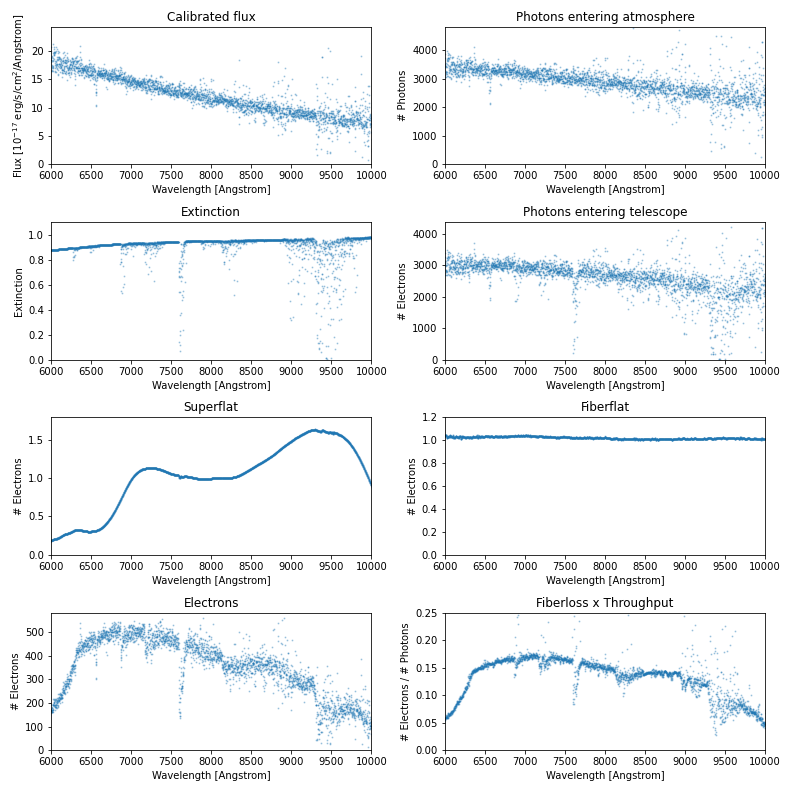
\includegraphics[width=14cm]{images/specsim/fiberloss_chart_red.png}
\caption{Chart showing fiberloss x extinction. SPECTROPHOTO\_STD plate 7027, mjd 56448, fiber 97, band `red'.}
\label{fig:fiberloss_chart}
\end{figure}

\begin{figure}[h]
    \centering
    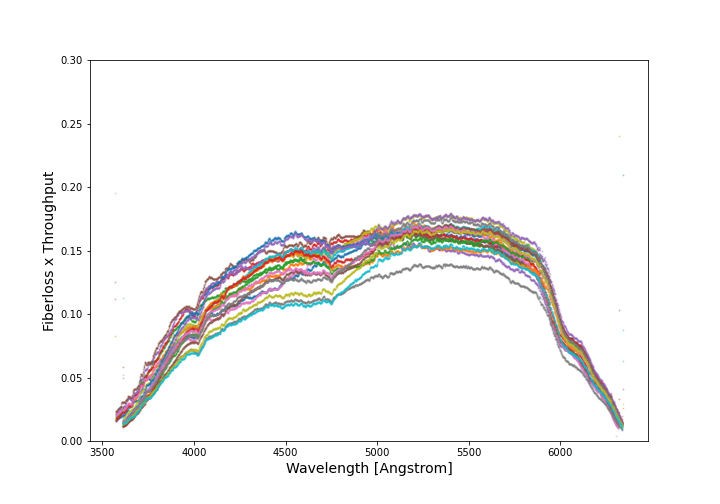
\includegraphics[width=0.495\textwidth]{images/specsim/all_standards_blue.png}
    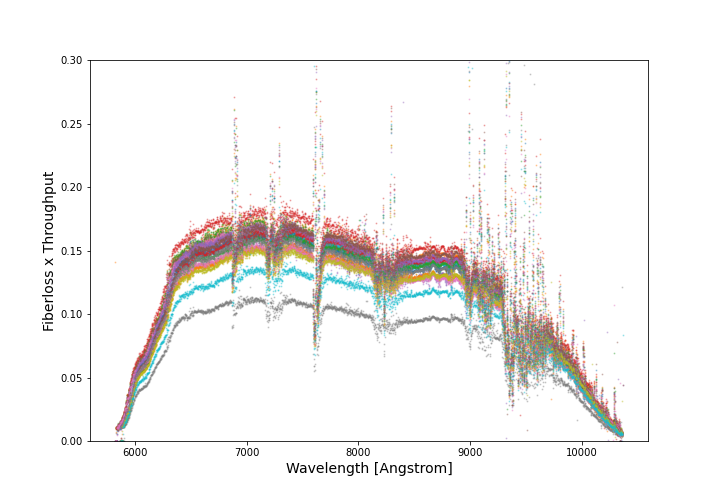
\includegraphics[width=0.495\textwidth]{images/specsim/all_standards_red.png}
    \caption{All standards on plate 7027, blue (left) and red (right).}
    \label{fig:all_stds}
\end{figure}

\begin{figure}[h]
    \centering
    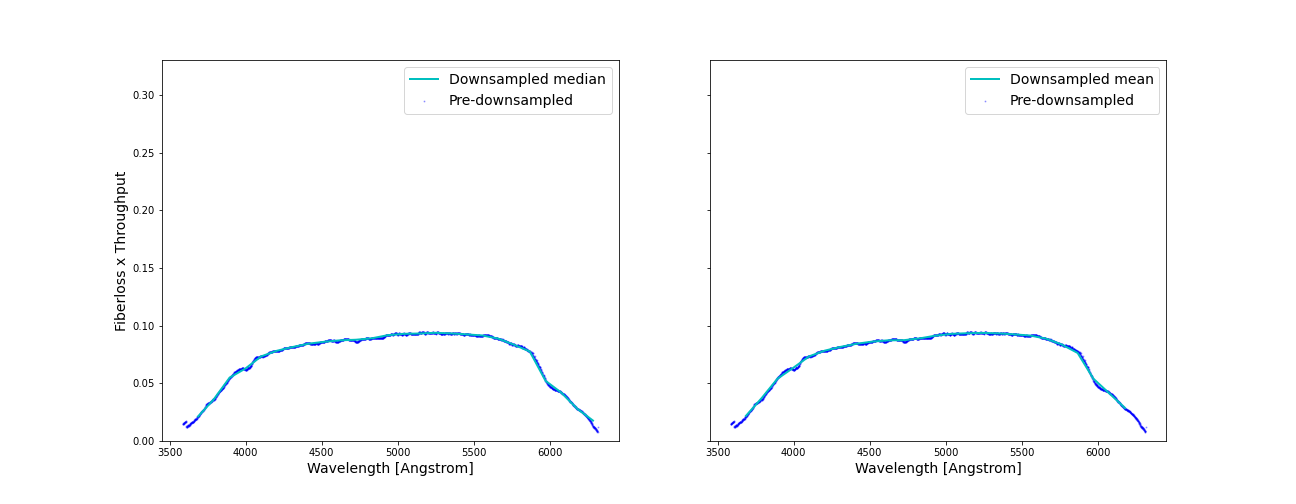
\includegraphics[width=20cm]{images/specsim/downsampled_blue.png}
    \caption{Median vs mean downsampled of all SPECTROPHOTO\_STD blue camera.}
    \label{fig:downsampled_blue}
\end{figure}


\begin{figure}[h]
\centering
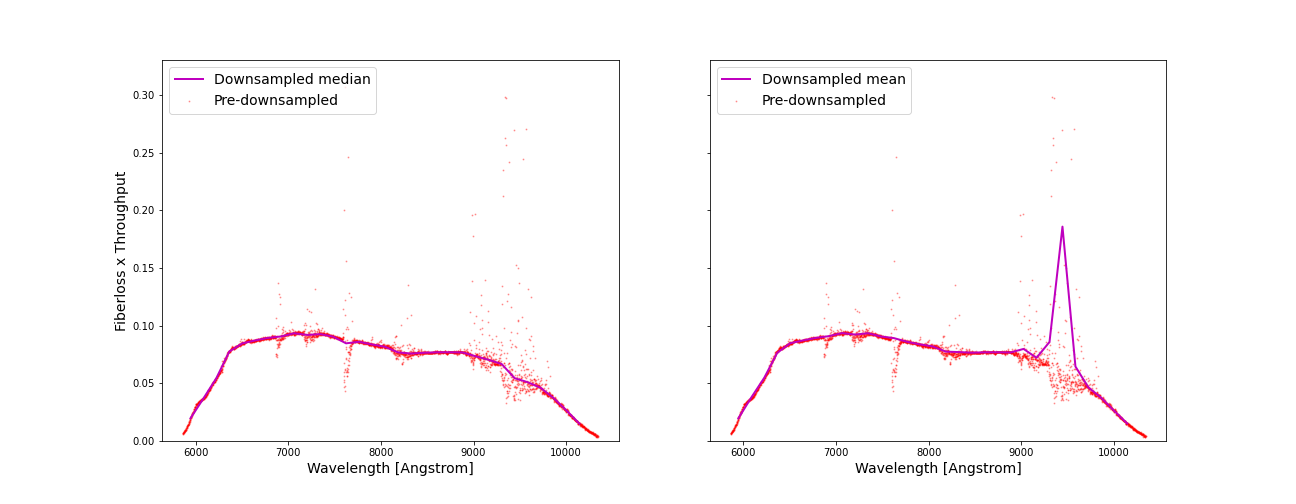
\includegraphics[width=20cm]{images/specsim/downsampled_red.png}
\caption{Median vs mean downsampled of all SPECTROPHOTO\_STD red camera.}
\label{fig:downsampled_red}
\end{figure}

This quantity was derived for all standard stars on plate 7027 listed in Table \ref{tab:eboss_plates}, the result of which is shown in Fig. \ref{fig:all_stds}. Next, the median over all 20 standard stars on this plate was taken, and smoothing was applied by downsampling by a factor of 100. The product of the fiberloss and the throughput after smoothing is shown in Figs. \ref{fig:downsampled_blue} \& \ref{fig:downsampled_red} for the blue and red cameras, respectively. 


\begin{figure}[h]
\centering
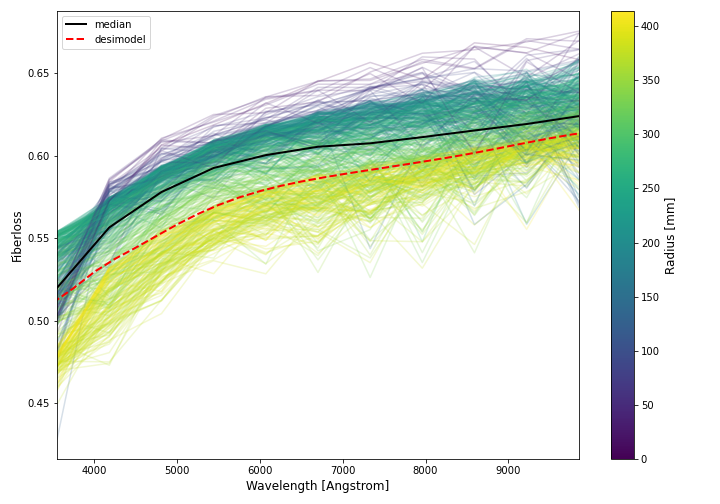
\includegraphics[width=14cm]{images/specsim/desimodel-qso-fiberloss.png}
\caption{Simulated fiberloss (galsim + desimodel).}
\label{fig:desimodel_qso_floss}
\end{figure}


The final eBOSS throughput data was obtained by dividing out a constant value for the fiberloss. Fig. \ref{fig:desimodel_qso_floss} shows fiberloss values as a function of wavelength for 500 simulated DESI quasars, with the median over all fibers shown in the black solid line and the tabulated quasar fiberloss values shown in the dashed red line. The different fiber colors correspond to distance from the center of the focal plane. It was decided that a fiber acceptance value of 0.55 would be sufficient to use, as this seemed to be about the average across all wavelengths.

At one point it was found that data for the expected throughput of the eBOSS spectrograph was available from \cite{Smee_2013}, shown as the black line in Fig. \ref{fig:smee}. Fresnel losses at the fiber faces, focal ration degredation, and ``slit" losses for 1" FWHM seeing conditions modeled with a double Gaussian PSF are not shown in this curve and had to be accounted for and degraded the final throughput curve by an additional 15\%, 4\%, and 17\%, respectively. A comparison of the throughput derived from standards stars on plate 7027 versus the expected throughput data provided by the eBOSS collaboration is shown in Fig. \ref{fig:throughput}. The latter was ultimately used for the specsim eBOSS configuration.


\begin{figure}[h]
\centering
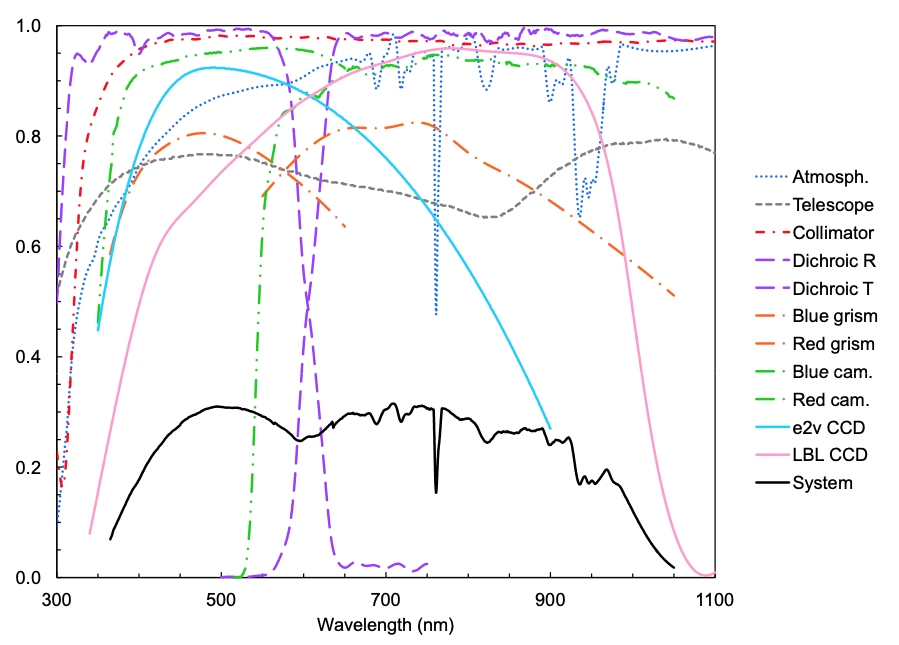
\includegraphics[width=14cm]{images/specsim/smee_throughput.png}
\caption{Expected eBOSS throughput from Smee et al.}
\label{fig:smee}
\end{figure}

\begin{figure}[h]
\centering
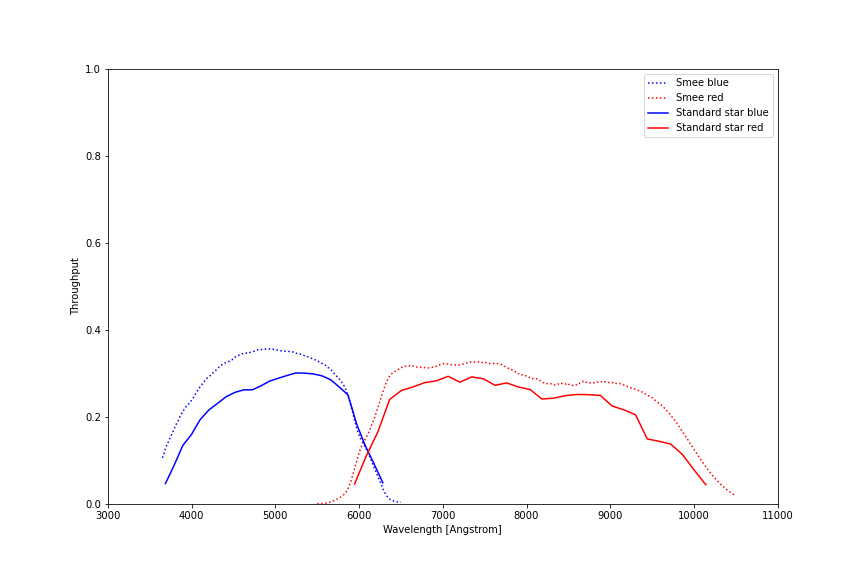
\includegraphics[width=14cm]{images/specsim/throughput_7027_56448.png}
\caption{Final throughput comparison.}
\label{fig:throughput}
\end{figure}


\subsubsection{Fiber acceptance fraction}

The fiber acceptance fraction, or fiberloss, is the fraction of light incident on the fiber that makes it through the fiber face. It is ultimately determined by the source profile, as the total light extended sources is less likely to pass through the fiber than light from sources with star-like profiles, such as quasars.

There are three different methods to account for fiberloss in \pkg{specsim}. The \pkg{table} method uses a pre-computed table of fiberloss fractions based on the source type. The \pkg{galsim} method uses information about the transverse profile of the source on the sky to calculate fiberloss fractions via \pkg{GalSim}, a software package that simulates high-fidelity images of galaxies (cite). Finally, \pkg{specsim} can interpolate fiber acceptance values pre-computed with \pkg{GalSim} with the \pkg{fastsim} method. This method assumes a fixed axis ratio of 0.7, a fixed Moffat PSF model with $\beta=3.5$ for the atmosphere, and a fixed fiber diameter of $107 \mu$m. 



\begin{figure}[h]
    \centering
    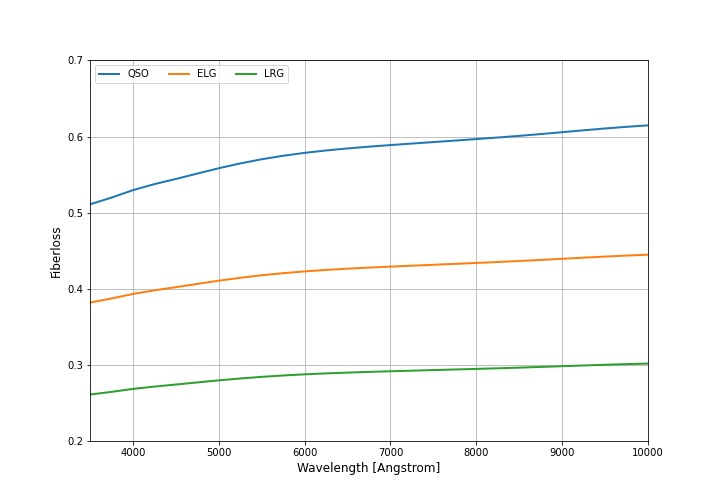
\includegraphics[width=0.495\textwidth]{images/specsim/desimodel-fiberloss.png}
    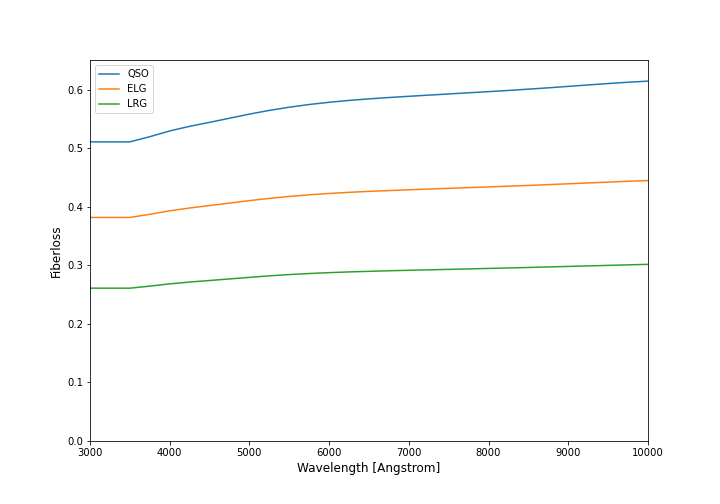
\includegraphics[width=0.495\textwidth]{images/specsim/eboss_fiberloss.png}
    \caption{Quasar fiberloss for eBOSS (right), adjusted from DESI(left).}
    \label{fig:qso_fiberloss}
\end{figure}



%Extinction

\begin{figure}[h]
\centering
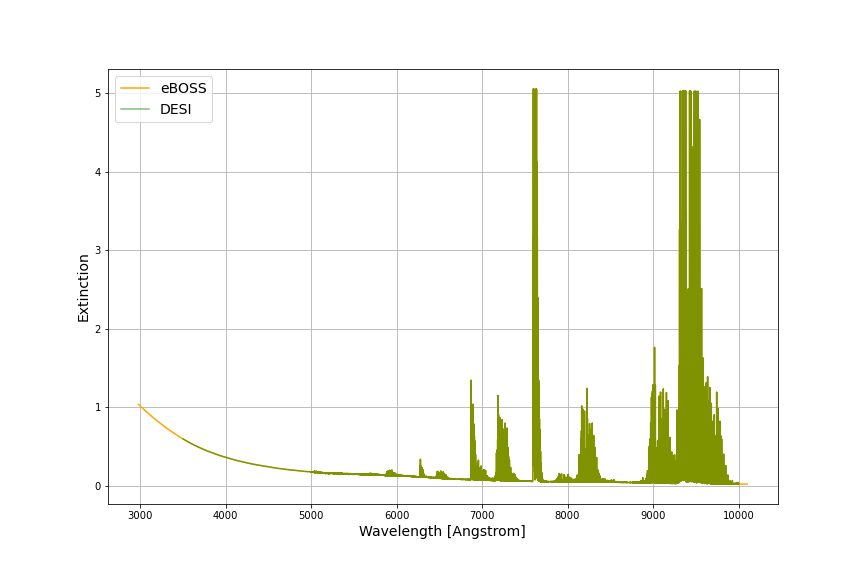
\includegraphics[width=12cm]{images/specsim/extinction.png}
\caption{Extinction comparison.}
\label{fig:extinction}
\end{figure}

%Sky brightness

\begin{figure}[h]
\centering
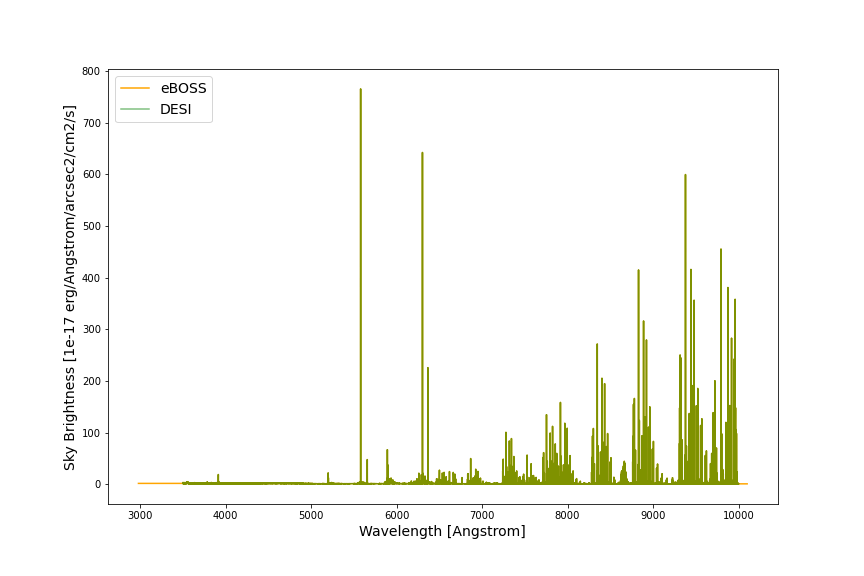
\includegraphics[width=12cm]{images/specsim/sky_brightness.png}
\caption{Sky brightness comparison.}
\label{fig:sky_brightness}
\end{figure}

%Source

\begin{figure}[h]
\centering
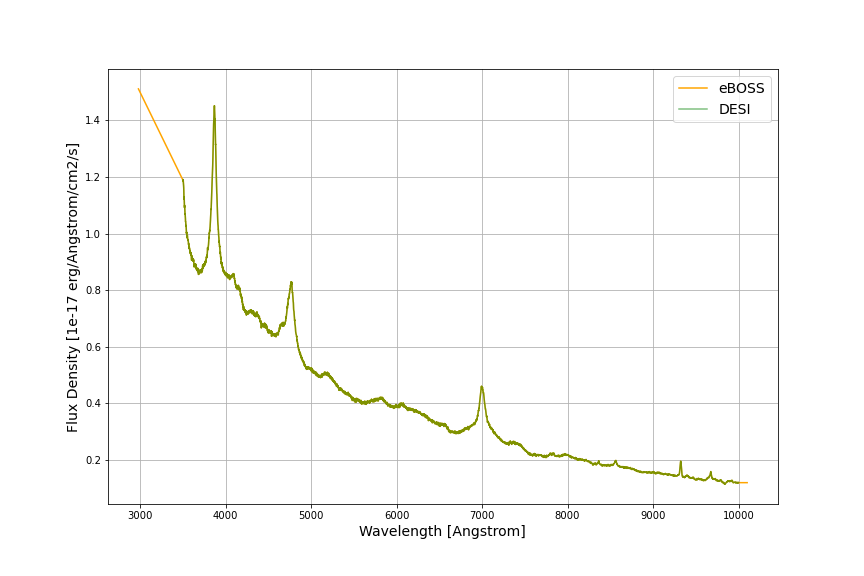
\includegraphics[width=12cm]{images/specsim/source.png}
\caption{QSO source comparison.}
\label{fig:qso_source}
\end{figure}

%Final config

\begin{figure}[h]
\centering
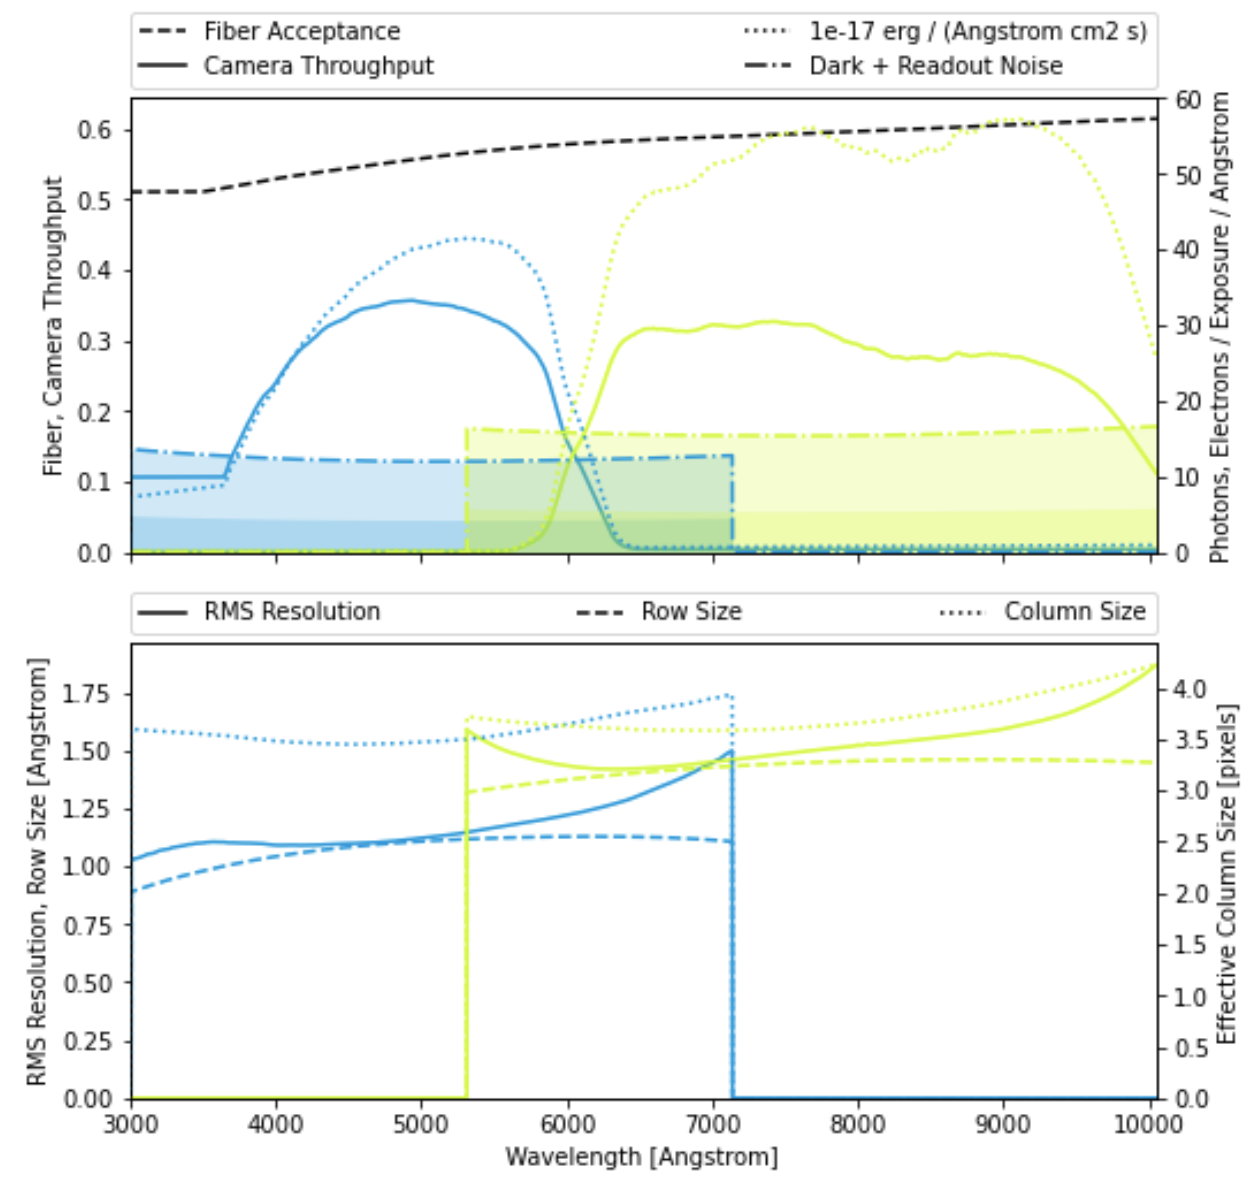
\includegraphics[width=12cm]{images/specsim/eboss_config.png}
\caption{eBOSS instrument configuration.}
\label{fig:eboss_config}
\end{figure}

\begin{figure}[h]
\centering
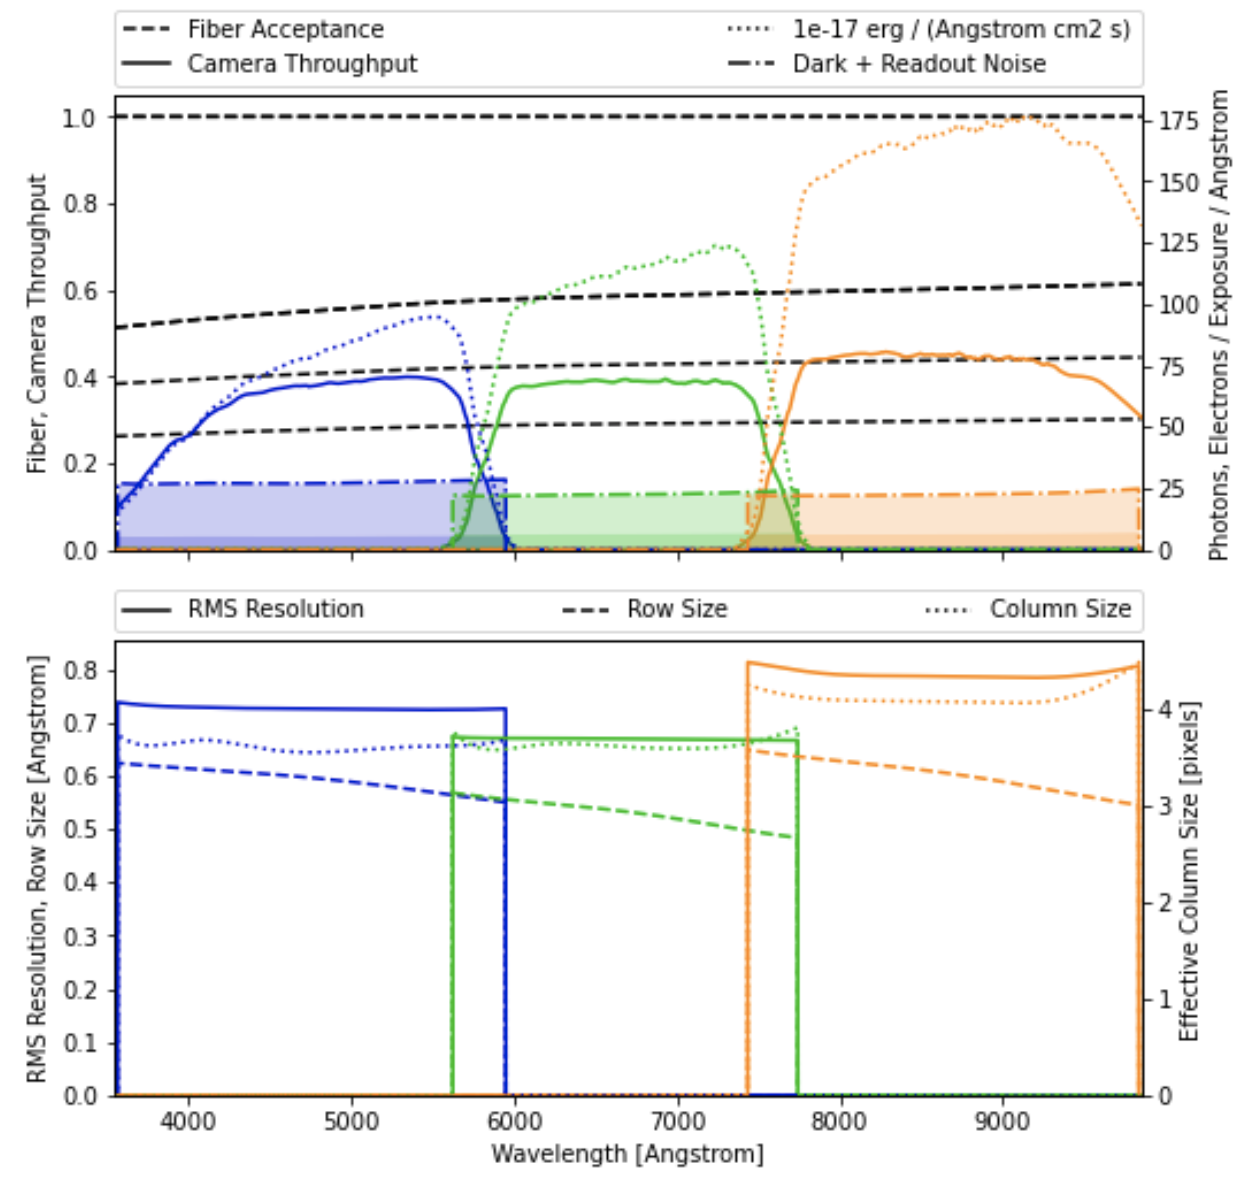
\includegraphics[width=12cm]{images/specsim/desi_config.png}
\caption{DESI instrument configuration.}
\label{fig:desi_config}
\end{figure}

\subsection{Verification/simulation}

\begin{figure}[h]
    \centering
    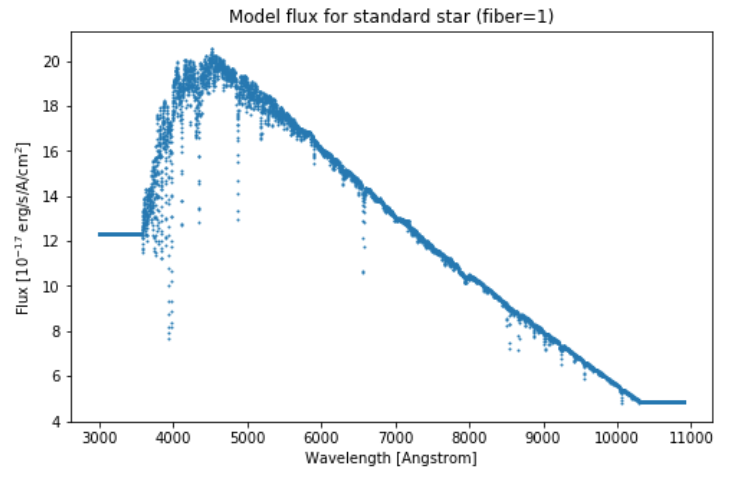
\includegraphics[width=0.495\textwidth]{images/specsim/stellar_model_4055_55359_1.png}
    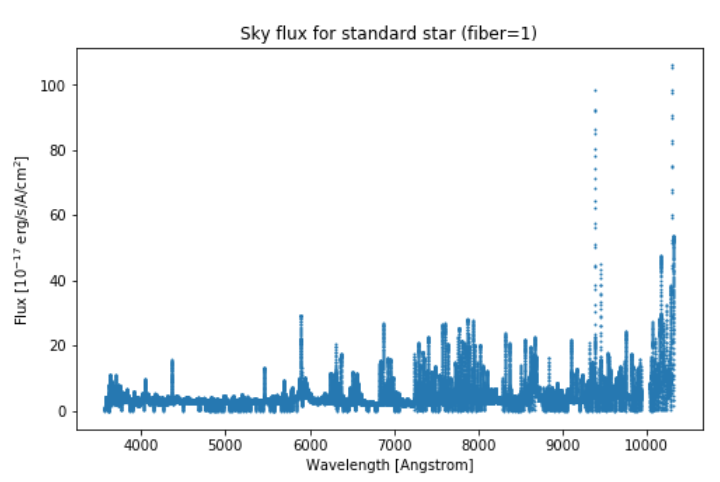
\includegraphics[width=0.495\textwidth]{images/specsim/sky_flux_4055_55359_1.png}
    \caption{Stellar model + sky data}
    \label{fig:star_sky}
\end{figure}


\begin{figure}[h]
\centering
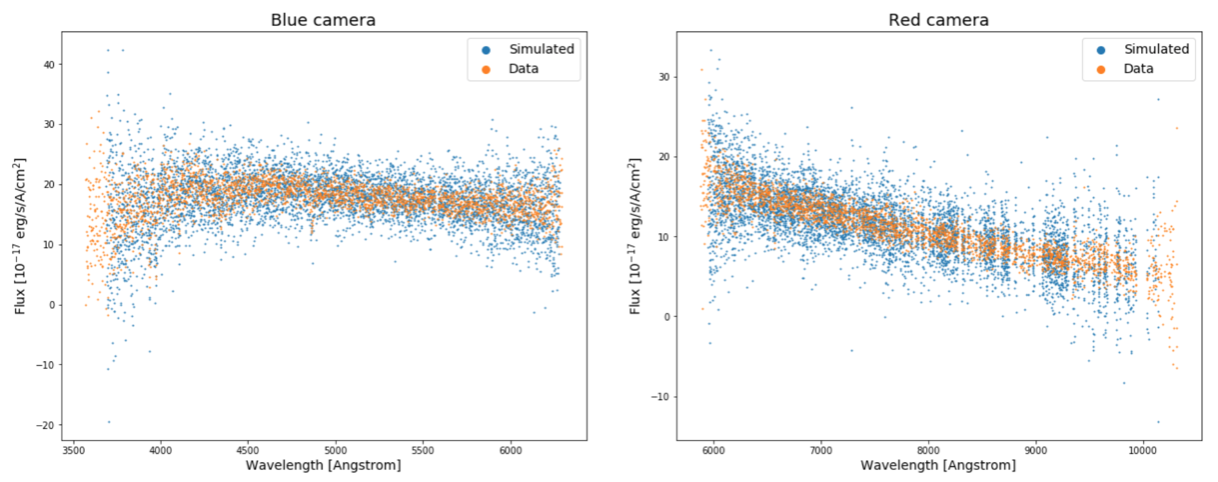
\includegraphics[width=17cm]{images/specsim/simulated_output_4055_55359_1.png}
\caption{Simulated output.}
\label{fig:simulated_flux}
\end{figure}

\begin{figure}[h]
\centering
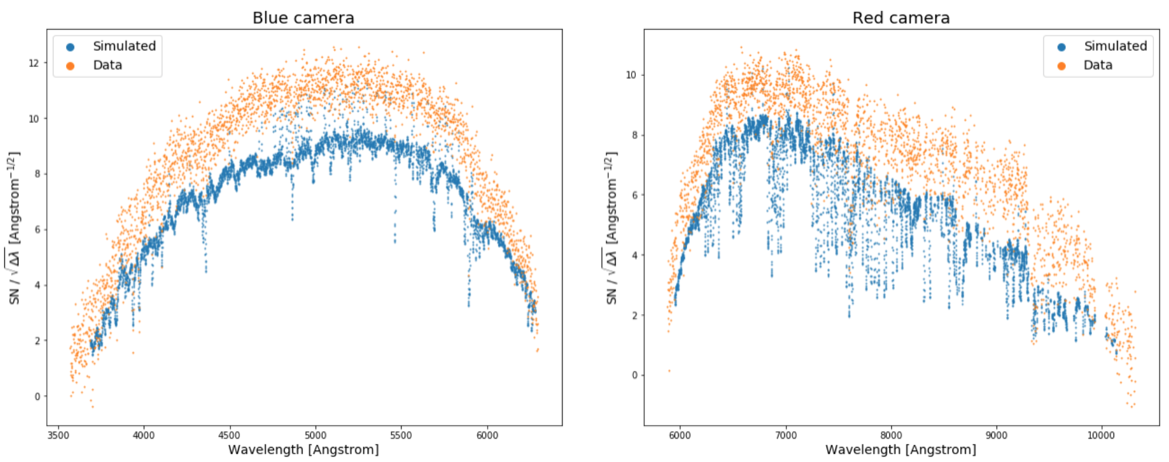
\includegraphics[width=16cm]{images/specsim/ivar_4055_55359_1.png}
\caption{Simulated ivar.}
\label{fig:simulated_ivar}
\end{figure}

\begin{figure}[h]
    \centering
    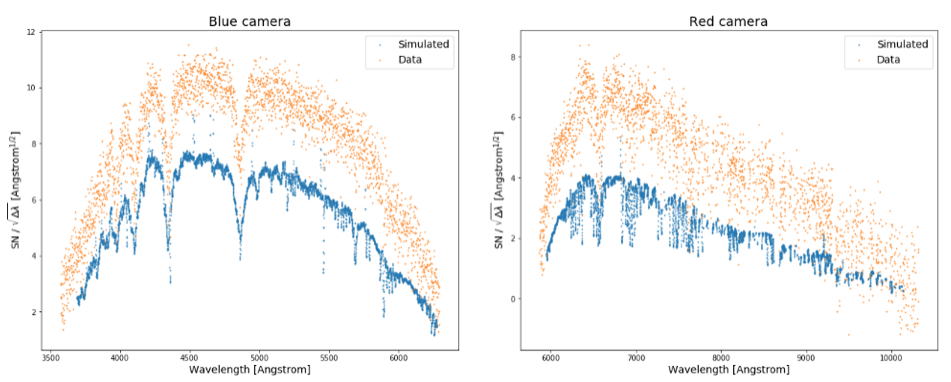
\includegraphics[width=0.495\textwidth]{images/specsim/ivar_4055_55359_334.png}
    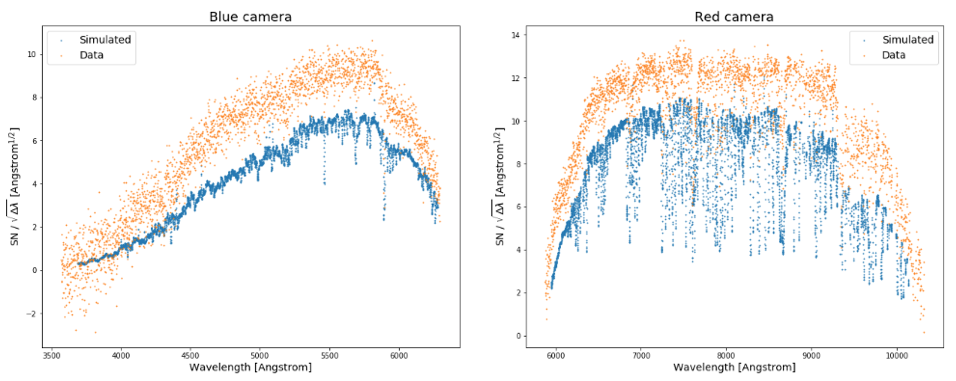
\includegraphics[width=0.495\textwidth]{images/specsim/ivar_4055_55359_395.png}
    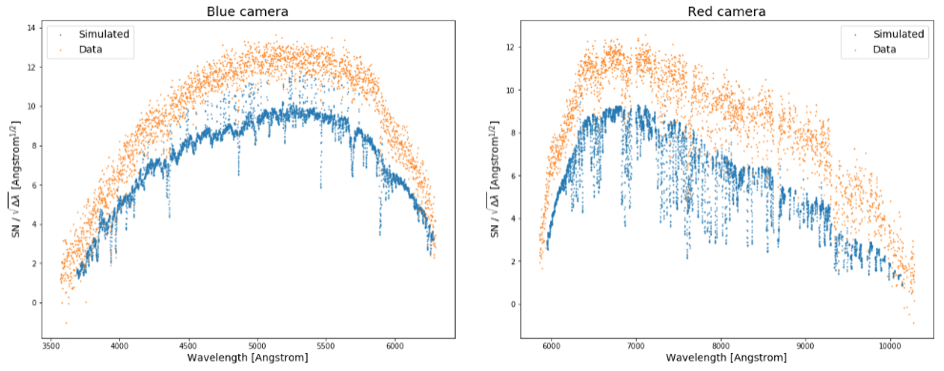
\includegraphics[width=0.495\textwidth]{images/specsim/ivar_4055_55359_41.png}
     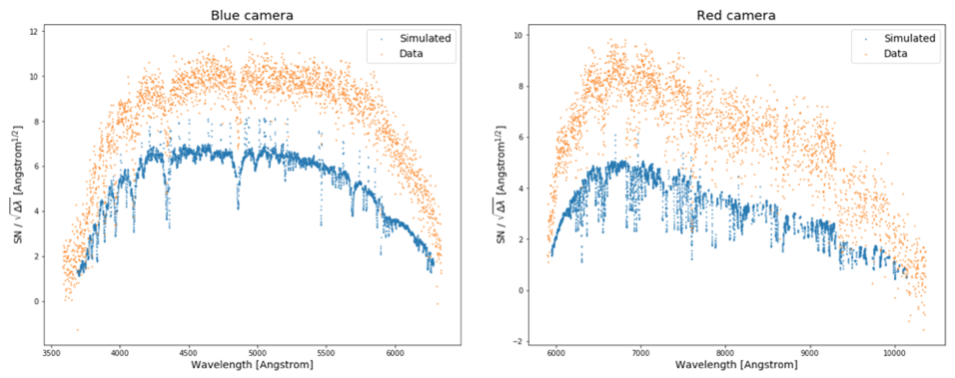
\includegraphics[width=0.495\textwidth]{images/specsim/ivar_4055_55359_694.png}
      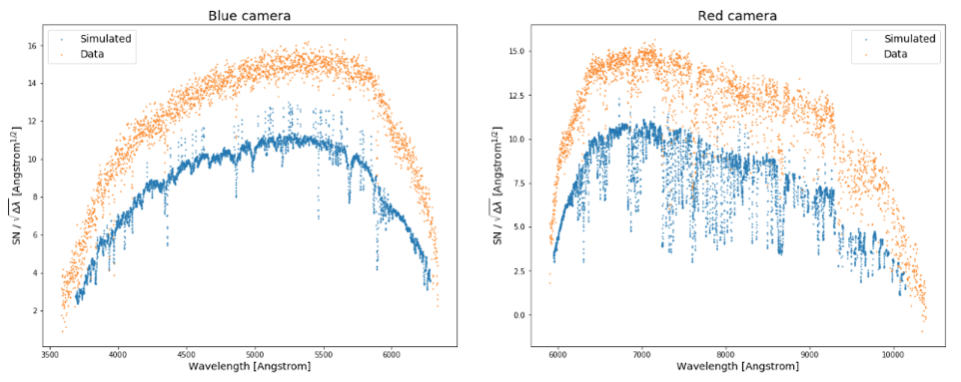
\includegraphics[width=0.495\textwidth]{images/specsim/ivar_4055_55359_890.png}
       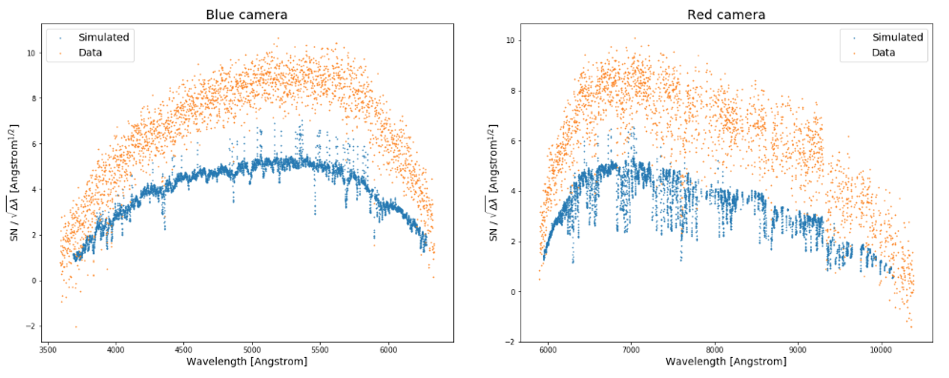
\includegraphics[width=0.495\textwidth]{images/specsim/ivar_4055_55359_970.png}
    \caption{ivar comparisons.}
    \label{fig:ivar}
\end{figure}

\begin{figure}[h]
\centering
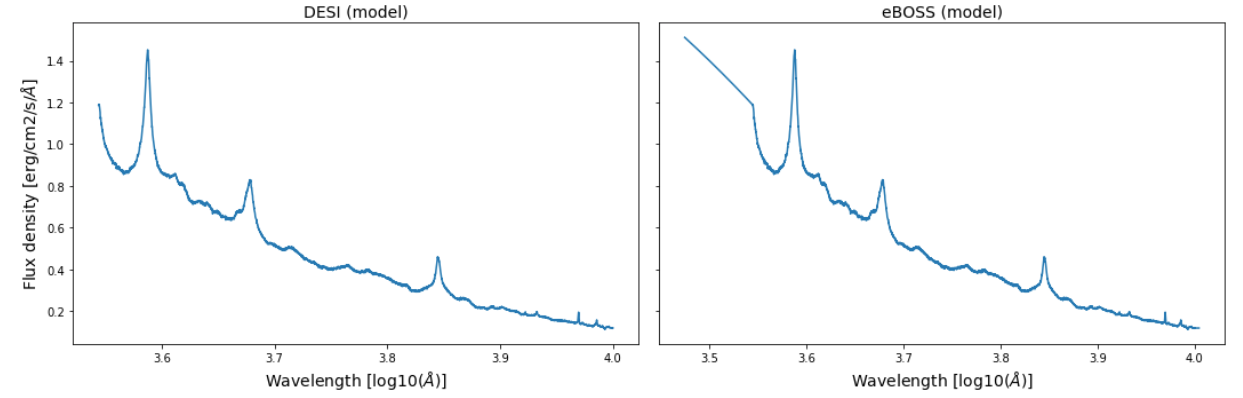
\includegraphics[width=16cm]{images/specsim/model_comparison.png}
\caption{Compare desi and eboss model qso spectrum.}
\label{fig:model_comparison}
\end{figure}

% mention how to produce these by calling specsim.simulator and specsim.simulate etc. a la: https://specsim.readthedocs.io/en/stable/output.html

\begin{figure}[h]
\centering
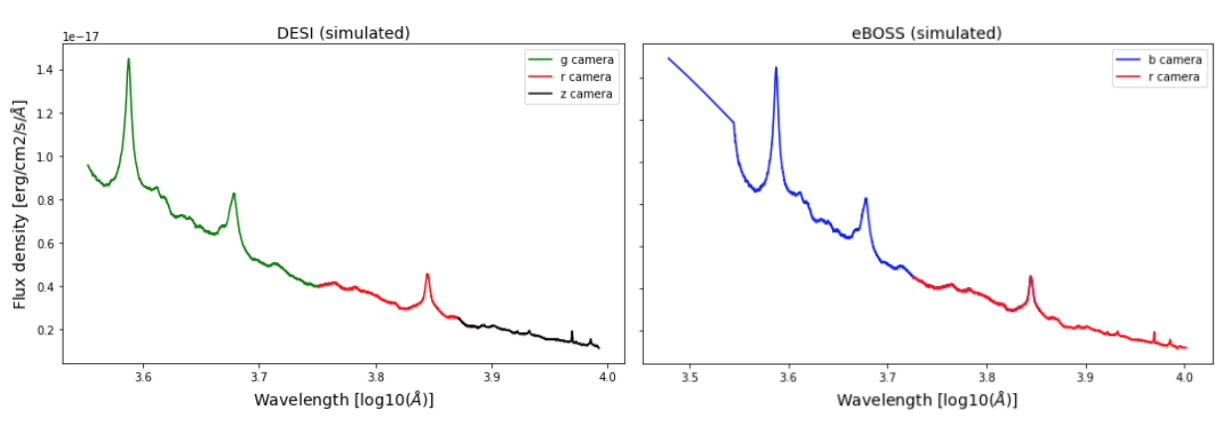
\includegraphics[width=16cm]{images/specsim/sim_comparison.png}
\caption{Compare desi and eboss simulated qso spectrum.}
\label{fig:sim_comparison}
\end{figure}

\begin{figure}[h]
\centering
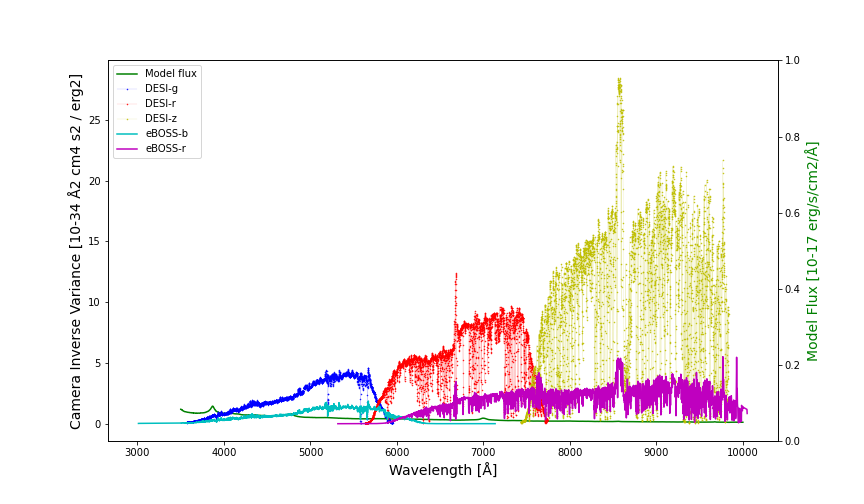
\includegraphics[width=16cm]{images/specsim/ivar_comparison.png}
\caption{Compare desi and eboss inverse variance.}
\label{fig:ivar_comparison}
\end{figure}

\section{Verifying the \pkg{specsim} sky model}

% specsim model based on eso? compare specsim sky brightness against empirical data from DECam
% mention all contributions to sky brightness: scattered moonlight, zodiacal light, extinction (photons scattered / absorbed
% due to molecules in the atmosphere, transparency / cloud cover

\begin{figure}[h]
    \centering
    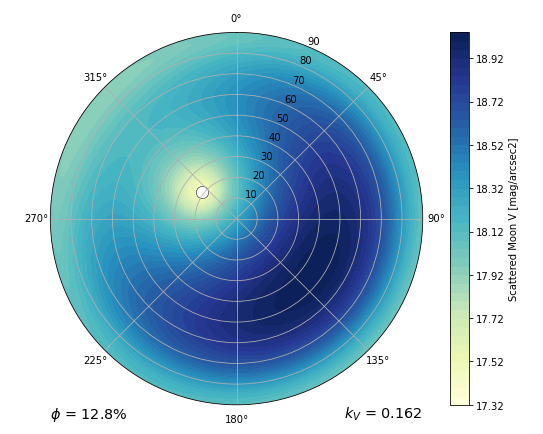
\includegraphics[width=0.495\textwidth]{images/specsim/lunar_plot_zen_21.21_az_307.76_ph_0.13.png}
    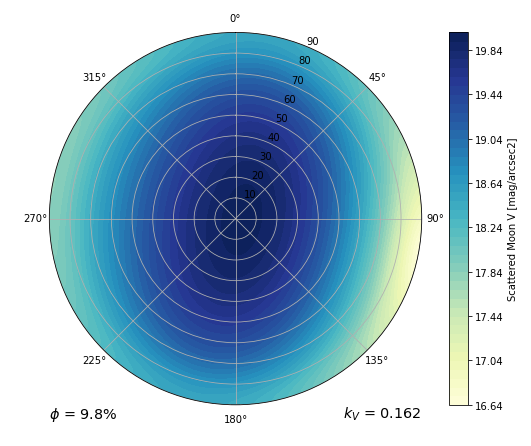
\includegraphics[width=0.495\textwidth]{images/specsim/lunar_plot_zen_97.31_az_100.50_ph_0.10.png}
    \caption{Lunar plots.}
    \label{fig:lunar}
\end{figure}

\begin{figure}[h]
\centering
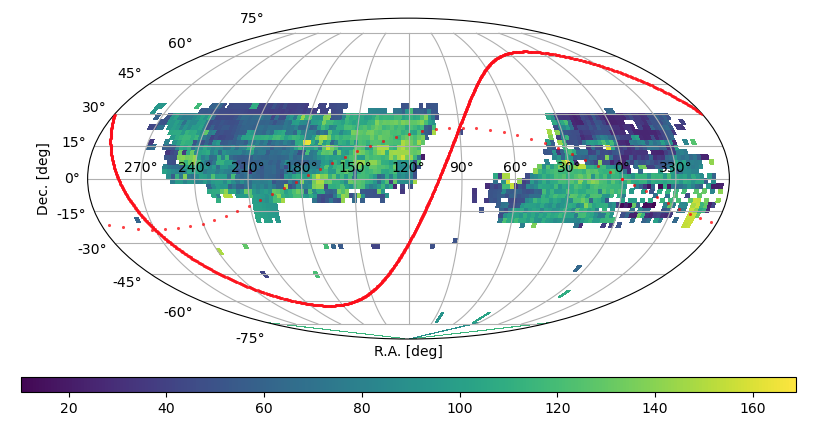
\includegraphics[width=16cm]{images/specsim/moon_separation_binned.png}
\caption{Moon separation.}
\label{fig:moon_sep}
\end{figure}

\begin{figure}[h]
\centering
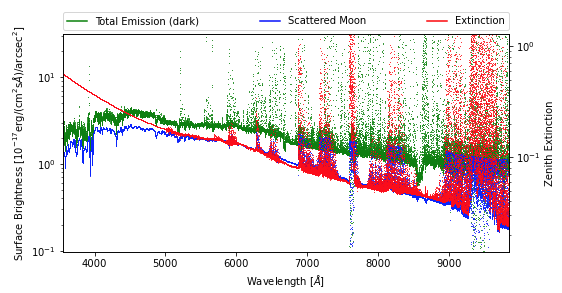
\includegraphics[width=16cm]{images/specsim/atmosphere_am_1.38_moon_zenith_63.28_sep_angle_53.24_moon_phase_0.45.png}
\caption{Contribution of different atmospheric components.}
\label{fig:atm_components}
\end{figure}

\begin{figure}[h]
\centering
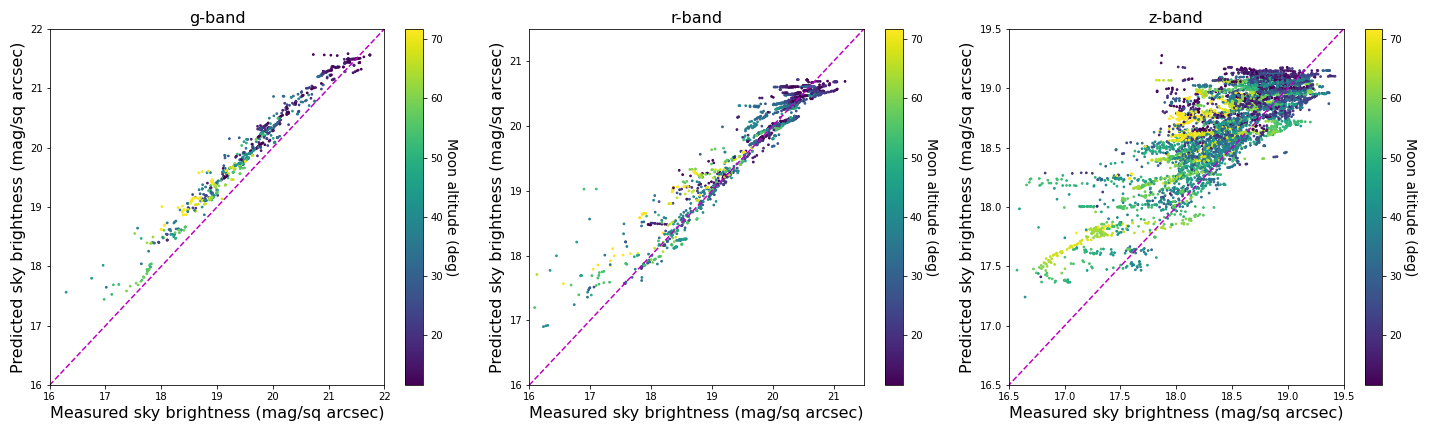
\includegraphics[width=18cm]{images/specsim/moon_brightness.png}
\caption{Predicted vs empirical sky brightness.}
\label{fig:sb_comparison}
\end{figure}

\begin{figure}[h]
\centering
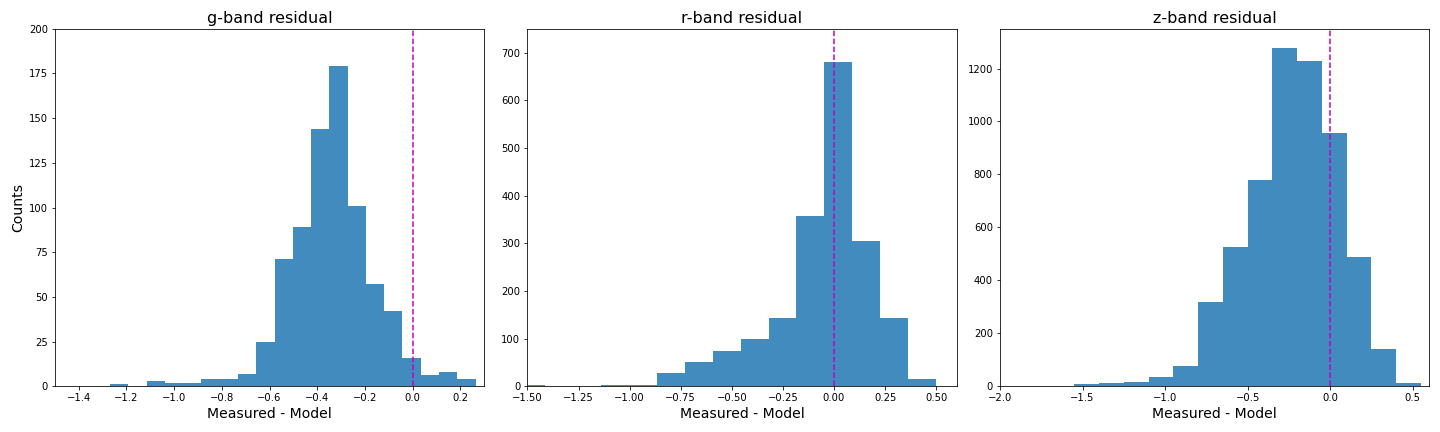
\includegraphics[width=16cm]{images/specsim/sky_brightness_residuals.png}
\caption{Sky brightness residuals predicted - model.}
\label{fig:sb_res}
\end{figure}


%%% Local Variables: ***
%%% mode: latex ***
%%% TeX-master: "thesis.tex" ***
%%% End: ***
